%-------------------------------------------------------------------------------
\chapter{Deep Learning platformok}
%-------------------------------------------------------------------------------
\section{hybrid deep learning} \label{sect:hybridDL}
%hybrid computing
A mai nagy teljesítményű párhuzamos számítási rendszerek igyekeznek kiaknázni az eltérő architektúrájú processzorok együttes alkalmazásában rejlő lehetőséget. Az ilyen heterogén rendszerek nemcsak nagyobb számítási kapacitással rendelkeznek, --~összehasonlítva az homogén rendszerek egy processzormagra eső számítási teljesítményét~-- de jelentősen kisebb az energiafelhasználásuk. Rengeteg területen alkalmaznak ilyen rendszereket, többek között elektrontomográfiás képrekonstrukciónál\cite{agulleiro2012} párhuzamos számítást igénylő tudományos alkalmazásokhoz\cite{meredith2011} és az ún. \emph{smart manufacturing} gyártástechnológia esetén.\cite{li2019}

A párhuzamos adatfeldolgozás miatt ezek a rendszerek elsősorban grafikus processzor architektúrákat --~konkrétan \emph{általános célú grafikus processzorokat} (GPGPU)~-- alkalmaznak hagyományos CPU-k mellett.\footnote{Hibrid számítási rendszereknél előfordul még az FPGA-k és a DSP-k használata is.} Sok olyan rendszer épült korábban, ahol pár általános célú processzor mellett több GPGPU működött, azonban a legtöbb ilyen rendszer esetében a CPU-k pusztán az operációs rendszer futtatásában és számítási feladatok szétosztásában vett részt. Mély tanulás esetén előfordulhatnak olyan feladatok, amiket több CPU magra lehetne bízni.

A következő alfejezetekben szeretnék bemutatni olyan szoftvereket és hardvereket, melyek lehetséges építőkövei egy ilyen mély tanulásra használható hibrid számítási rendszernek.
%TODO konzultálj

\section{nGraph}
Az \ref{sect:hybridDL}~alfejezetben említett hibrid számítási rendszereken a neurális hálózatok működtetése nehézkes feladat. Szükséges a neurális hálózatból származtatható számítási gráf optimalizálása a különböző processzor architektúrákra, hogy képesek legyünk kihasználni a több architektúra adta sebességnövekedést. Többek között erre a célra az Intel belekezdett az nGraph projekt fejlesztésébe. Az nGraph hivatalos dokumentációja részletesen leírja, hogy a fejlesztők milyen problémák megoldására tervezték ezt a szoftvert.\cite{web:ngraph_intro}.

Az nGraph az Intel által fejlesztett programkönyvtár és egy futtatási környezet/fordító készlet melyet mély tanuló projektekhez terveztek.
Legszembetűnőbb tulajdonsága, hogy képes többféle hardver architektúrán futtatni és beépíthető számos keretrendszerbe.
Ezek azok a jellemzők, amiket kerestünk témavezetőmmel, hogy mély tanulást tudjunk végeztetni hatékonyan a \emph{HuSSar-on}. 
Ezen túlmenően a jövőbeli fejlesztések az iparban egyre jelentősebben igényelik, hogy a modern MI rendszerek skálázhatóak legyenek, mert egyrészt a neurális hálók egyre komplexebbé válnak, másrészt az általuk feldolgozott adatok mennyisége is rohamosan növekszik. Jelenleg két bevett gyakorlat van a mély tanulás felgyorsítására:
\begin{enumerate}[noitemsep]
	\item \textbf{Dedikált hardver tervezése a mély tanulással kapcsolatos számításokhoz} -- Sok vállalkozás tervez \emph{Alkalmazásspecifikus integrált áramköröket} (ASIC) neurális hálózatok betanítására és futtatására.
	\item \textbf{Szoftver optimalizáció} -- Programkönyvtárakat tartalmazó fejlesztési keretrendszerek fejlesztése, melyek képesek a hálózatokkal kapcsolatos számításokat több szálon, optimalizáltan futtatni. Az nGraph, mint fordító is egy ilyen megoldás.
\end{enumerate}

\subsection{Motiváció}
A mai legmodernebb szoftveres megoldás mély tanulásra az, ha integrálunk kernel könyvtárakat\footnote{Programkönyvtár, mely neurális hálókkal kapcsolatos elemi, \emph{mag} függvényeket tartalmazzák} mély tanulási keretrendszerekbe.
Ilyen integráció lehet például ha a Tensorflow keretrendszer alatt az Nvidia CuDNN könyvtárát használjuk.
A {kernel könyvtárak} egy adott célarchitektúrára optimalizált kernelekből és egyéb műveleti szintű optimalizálásokból állnak, ezekkel érve el teljesítménynövekedést.
Azonban a kernel könyvtáraknak három fő problémája van:
\begin{enumerate}
	\item Nem biztosítanak gráf szintű optimalizálást
	\item A keretrendszerek integrációja a {kernel könyvtárakkal} nem skálázható
	\item A szükséges lefordított kernel könyvtárak száma növekszik, ahogy új processzorok jelennek meg
\end{enumerate}
Az nGraph fordító megoldás az első két problémára, és a \emph{PlaidML}-el ötvözve kiküszöbölhető a harmadik probléma.
\subsection{Gráf szintű optimalizálás}
Az nGraph dokumentációjában áll egy példa arra vonatkozóan, hogyan lehet, hogy egy mély tanulási keretrendszer integrálva egy {kernel könyvtárral} a számításokat optimálisan végzi, mégis a számítási gráf a csúcsait alkotó műveletek szempontjából mégsem optimális.
\begin{figure}[h]
	\centering
	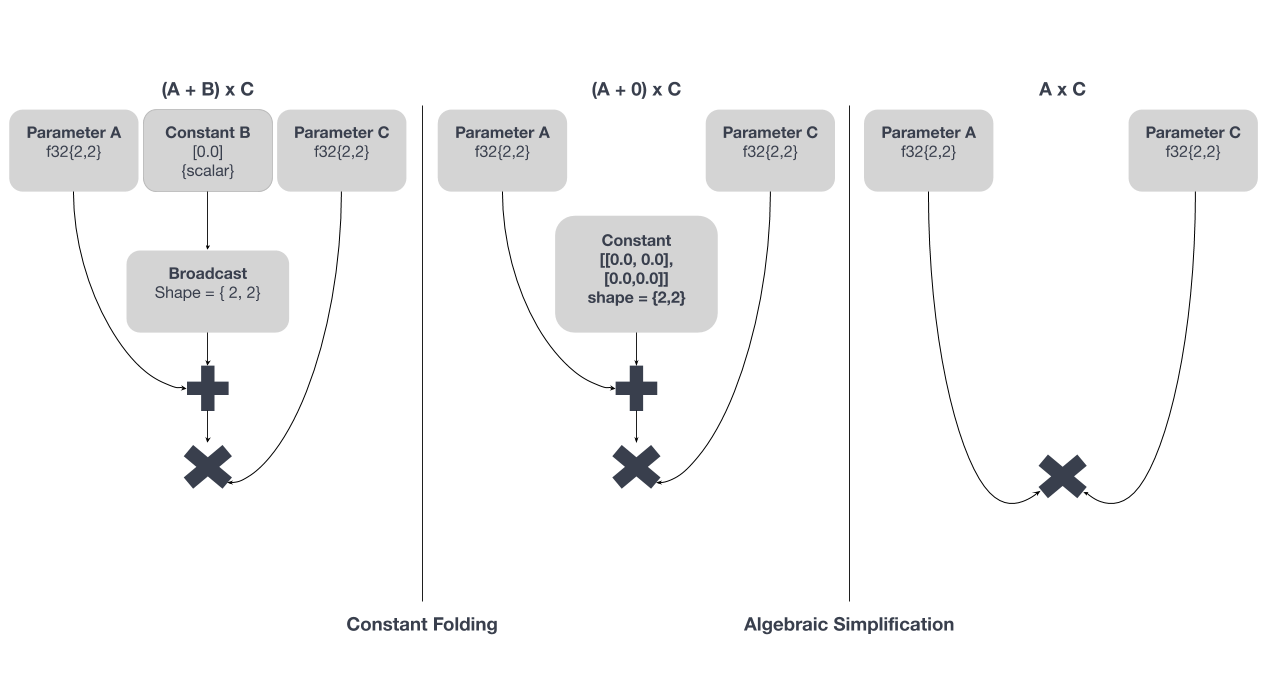
\includegraphics[width=0.9\textwidth]{kernel-problem-1.png}
	\caption{két optimalizálás módszer: konstans összehajtás és algebrai egyszerűsítés a gráfon. \footnotesize forrás: \cite{web:ngraph_intro}}
	\label{fig:grafoptimalizalas}
\end{figure}
A \ref{fig:grafoptimalizalas}~ábra bemutatja, hogyan egyszerűsíthetünk az $A$,$B$ és $C$ tenzorokat feldolgozó, $ (A+B)*C $ tenzorműveletet végrehajtó számítási gráfon.
Fordítási időben megállapítható, hogy $B$ egy skalár konstans, így a \emph{konstans összehajtásnak}\cite{wiki:constfold} nevezett optimalizálás elvégezhető, és a 2 dimenziós vektorrá való kiterjesztés művelete elhagyható (helyette inkább közvetlenül létrehozunk egy $2\times2$ tenzort).
Ebben a példában $B=0$ skalár volt, így a belőle létrejött tenzor egy nullmátrix, így az semleges a kifejezés kiértékelésének szempontjából.
\emph{Algebrai egyszerűsítést} végezve az $ (A+0)*C $ leegyszerűsíthető az $A*C$ kifejezésre, így összesen két csúccsal csökkentettük a gráfunkat.
Ez az optimalizáció tehát a számítási gráf szintjén lett elvégezve.
Így belátható, hogy a mély tanulási keretrendszerbe integrált kernel programkönyvtárak nem optimális futást végeznek, hiába a műveletek szintjén elért optimalizálás.

\subsection{Skálázható keretrendszer integráció}
Ahogy gyarapodik a mély tanuláshoz használható gyorsítókártya architektúrák és keretrendszerek száma, a meglévő mély tanulást alkalmazó fejlesztési platformok bővítése egyre több munkát igényel és egyre nő a hibák megjelenésének a valószínűsége. Az integráció kapható készen, szakértő fejlesztőcsapatoknak kell implementálnia.
Minden új keretrendszert manuálisan kell integrálni a meglévő hardverek kernel könyvtárával és minden újonnan megjelenő hardvercsalád meghajtó programkönyvtárát be kell integrálni egyesével a meglévő keretrendszerekbe.
Ez a munka önmagában is hatalmasra tud nőni, de egy sok eszközből álló összeállítás nagyon törékeny és költséges a fenntartása.
Az nGraph úgy oldja meg ezt a problémát, hogy ún. \emph{hidakat} alkalmaz, amikkel integrálható valamelyik mély tanulási keretrendszerbe.
A híd megkapja a keretrendszerben megalkotott számítási gráfot vagy ahhoz hasonló struktúrát és átalakítja egy ún. \emph{közbenső reprezentációvá}\footnote{IR: Intermediate Representation}. Ezzel kaptunk egy egységes, platformfüggetlen számítási gráfot, így nem kell egy új programkönyvtárat beintegrálni minden egyes meglévő keretrendszer alá, elegendő csak az, hogy az nGraph-ban, mint programkönyvtárban implementált \emph{primitív műveleteket} támogassa az új programkönyvtár.

\subsection{Növekvő kernel szám}
Egy kernel könyvtár integrálása egyszerre több mély tanulási keretrendszerrel nehéz feladat és egyre komplexebbé válik, ahogy növekszik az optimális teljesítményhez szükséges kernelek száma.
Régen a mély tanulással kapcsolatos kutatások egy kis számú \emph{primitív} számítást használtak, mint a konvolúció, általános mátrixszorzás, stb. Az MI kutatás előrehaladtával és az ipari mély tanuló alkalmazások továbbfejlesztésével, a szükséges kernelek száma (k) exponenciálisan nő.
Ez a szám a processzor architektúrák számán (h), adattípusokon (t), műveleteken (p) és az egyes paraméterek számosságán (p) alapul ($ k = h \times t \times m \times p $).
\begin{table}[!ht]
	\centering
	\begin{tabular}{|c|c|c|c|}
		
		Hardver & Művelet & Adattípus & Paraméterek \\ 
		\hline
		CPU & konvolúció & 16 bites lebegőpontos & NCHW vagy NHWC \\ 
		
		GPU & MatMul & 32 bites lebegőpontos & 2D, 3D és 4D tenzorok \\ 
		
		FPGA & Normalizálás & 8 bites egész &  \dots \\ 
		
		\dots & \dots & \dots & \\
	\end{tabular} 
	\caption{Néhány példa, tényezőnként hányféle esetre kell külön fordítani  kernelt könyvtárt }
	\label{table:kernels}
\end{table}

Ezen probléma megoldásához jön képbe a PlaidML. Ez egy \emph{tenzor fordító}\footnote{Olyan fordító, melynek nyelve arra lett fejlesztve, hogy főleg tenzorműveleteket igénylő algoritmusokat tudjunk hatékonyan programozni\cite{wiki:plaidml}}, mely azt célozza, hogy képes legyen neurális hálózatokat tanítani és futtatni bármilyen típusú hardveren. Más szavakkal segíti a magas szintű keretrendszerek (Keras, ONNX, nGraph) integrálni olyan ezsközökkel, melyekhez nincs meg a szükséges támogatás vagy a meglévő szoftverkészlet hozzájuk szigorúan linceszelt.\cite{github:PlaidML}\cite{web:PlaidML}

Az nGraph tehát integrálható a PlaidML-el. Elsősorban az nGraph a platform független IR-rel igyekszik orvolsoni a skálázható backend-el kapcsolatos kihívást. A PlaidML ezt megtámogatja azzal, hogy képes az IR-ből származó gráfokból LLVM, OpenCL, OpenGL, CUDA és Metal kódot generálni melyek a megfelelő hardveren futtathatóak. Így egy magas szintű keretrendszerben írt neurális háló lefordul Intel és AMD processzrokon valamint grafikus processzorokon, az nVidia processzorain, továbbá az Apple cég által feljelsztett eszközökön. Az nGraph gráf szintű optimalizációját ráadásul kiegészíti automatikusan a PlaidML alacsonyabb szinten, ezzel teljesítmény növekedést érve el.

Összegzésül tehát az nGraph feldarabolja a neurális hálózathoz tartozó számítási gráfot processzor architektúrának megfelelően, majd ezen gráfokat a PlaidML lefordítja a megfelelő kódokra, melyeket aztán a célprocesszorokra lefordítunk és futtatunk.

\section{Grafikus processzorok a mély tanulásban}
Változatos megoldások születnek a mély tanulás gyorsítására a hardvergyártók részéről. Kezdetben a nagy teljesítményű általános célú grafikus processzorokat (GPGPU) alkalmazták szinte kizárólag a neurális hálózatokkal kapcsolatos számításokhoz, mert ezek az architektúrák kifejezetten hatékonyan tudnak vektor és mátrixműveleteket végezni --~tulajdonképpen pont erre tervezték őket. Azonban ahogy elkezdett terjedni a mély tanulás olyan területeken is, ahol számít az alacsony hűtésigény, kiegyensúlyozott energiafogyasztás vagy a hordozhatóság, új architektúrák is kezdtek megjelenni. A következőkben bemutatok pár --~a mély tanulásban használt~-- hardvert és két szoftveres környezetet, melyek jól körvonalazzák, milyen irányba fog fejlődni a gépi tanulás technológiája.

\subsection{Nvidia által fejlesztett gyorsítókártyák}
Abban az időben mikor a mély tanulás bekerült a köztudatba a grafikus processzor gyártóknak olyan megoldásaik voltak, amikkel általános számítási feladatok programozását tette lehetővé a termékeiken. Ilyen az Nvidia CUDA (\emph{Compute Unified Device Architecture}) is, ami egy párhuzamos számítási platform és alkalmazásprogramozási interfész. Maga a platform egy olyan szoftverréteg, mely közvetlen hozzáférést enged a GPU utasításkészletéhez.\cite{wiki:cuda} Az API pedig olyan programozási eszközöket nyújt, amivel hatékonyan lehet CUDA képes GPU-n futó programot írni. A cég által közzé tett dokumentációk alapján nagy vonalakban bemutatnám a neurális hálózatok fejlesztéshez használható eszközeit.\cite{web:cudnn}
Ahhoz, hogy neurális hálózatokat futtassunk CUDA platform szükséges a CuDNN (\emph{CUDA Deep Neural Network Library}) könyvtárcsomag, mely a nélkülözhetetlen elemi függvényeket implementálja:
\begin{enumerate}
	\item Konvolúció
	\item Adatok összevonása (pooling)
	\item neuron aktivációs függvények
	\item tenzor transzformáció
%	\item LRN, LCN and batch normalization
\end{enumerate}
A CuDNN használatakor szükséges egy kezelőt (handler) inicializálni a \verb|cudnnCreate()| metódus hívásával. A metódus hívásával inicializálódik a programkönyvtár is, elvégzi a gazdarendszer és a gyorsítókártya erőforrásainak allokációját. Továbbá a visszaadott eszközkezelő mutat az inicializált gyorsítóra, így használható a későbbi függvényhívásoknál, melyeket az adott eszközön akarunk végrehajtatni.

A vállalat GPU-jainak magjai közül CUDA magoknak hívja azokat a speciális számítási egységeket, melyek egyedileg programozhatóak a platformon (tehát CUDA alatt nem utilizálható az összes mag). A mai legmodernebb gyorsítókártyákat az NVIDIA Turingnak nevezett architektúrájú processzorokkal szereli fel.
%Itt szeretnék bemutatni két felhasználási területük szempontjából eltérő kártyát:
Több fejlesztési irányt követnek a gyártók: Standard asztali és mobil grafikus processzorok, High-end asztali GPU (Nvidiánál: Quadro és TitanRTX\cite{spec:titan-rtx}), szerver oldali GPU (Tesla T4 \cite{spec:tesla-t4}), valamint kifejezetten HPC-re szánt GPU (Tesla v100\cite{spec:tesla-v100})

\paragraph{TITAN RTX}
%Turing microarchitecture (TU102)
%24~GB GDDR6 @ 1750~MHz
% bitráta 14~Gb/s
% sávszélesség 672~GB/s (384bites busz)
%órajel alap 1350~MHz, csúcs 1770~MHz
% 576~tenzor mag
% 4608~CUDA mag
% 32.62 TFLOPS (FP16) 2:1 arány
% 16.31 TFLOPS (FP32)
% 600~W felvett teljesítmény
% TDP: 280~W
Igen nagy teljesítményű grafikus kártya, mely a cég \emph{turing} mikroarchitektúrájú TU102 processzorral van felszerelve, ami 4608~CUDA processzormagot, valamint 576 tenzor magot tartalmaz és alapjáraton 1350~MHz órajelen üzemel. A kártyát felszerelték 24~GB GDDR6 memóriával, melynek sávszélessége 672~GB/s\footnote{a memóriaegységek 384~bit széles adatbuszon továbbítanak adatot 14~Gb/s-os bitrátával}. Elméleti számítási kapacitása 16.31~TFLOP/s (billió lebegőpontos művelet másodpercenként) egyszeres pontosságú lebegőpontos műveletek esetén. Ez az érték félszeres pontosság esetén --~amit a mai neurális hálózatoknál gyakran használnak~-- dupla ennyi. Ez egy nagy energiafogyasztású kártya, a gyártó 600~W teljesítmény leadására képes tápegységet ajánl az eszköz mellé.

\paragraph{Tesla T4}
%turing microarchitecture (TU104)
%16~GB GDDR6 @ 1250~MHz
% sávszélesség 320~GB/S (256bites busz)
% órajel alap 585~MHz, csúcs 1590~MHz
% 320~tenzor mag
% 2560~CUDA mag
% 65.13~TFLOPS (FP16) 8:1 arány
% 8.141~TFLOPS (FP32)
% 350~W felvett teljesítmény
% TDP: 70~W
Ezt a grafikus kártyát kifejezetten adatközpontok komponenseként szánták, ezért nem is szolgáltat videó jelet. Számítási teljesítményes is bizonyos szempontból szerényebb a TITAN RTX-nél. Szintén turing architektúrájú TU104 processzora 2560~CUDA magot tartalmaz. A szerényebb felszereltségnek ugyancsak az adatközponti felhasználása miatt van jelentőssége, hogy így kisebb áramfelvétel és hőleadás mellett tudjon üzemelni -- 350~W ajánlott leadási teljesítmény és összehasonlításképp a TITAN RTX \emph{Thermal Design Pointja} 280~W, míg ennek a kártyának csupán 70~W. Egyszeres pontosságú lebegópontos műveleteket alkalmazó számítások elméleti sebessége 8,141~TFLOP/s, viszont a félszeres pontosságnál nyolcszor gyorsabb, azaz ekkor 65,13~TFLOP/s az elméleti sebessége. Ebből látszik, hogy ez a kártya kifejezetten mély tanuláshoz és olyan alkalmazásokhoz lett optimalizálva, ahol félszeres pontosságú lebegőpontos számításokat kell végezni túlnyomó részt. A teljesség kedvéért megemlítem, hogy a kártya 16~GB szintén GDDR6 típusú memóriával lett felszerelve, melynek sávszélessége 320~GB/s (256~bites buszszélesség).

\paragraph{Tesla V100}
%v100 GPU NVlink kártya
% 16~vagy 32~GB HBM2 @ 1750~
% sávszélesség 900~GB/s (4096bites busz)
%640 tenzor mag
%5120 CUDA mag @ 1455~MHz 
% PCIe 32~GB/s
%14~TFLOP/s (FP32)
%NVLink 300~GB/s
%31,33~TFLOP/s (FP16)
%15,7~TFLOP/s (FP32)
A Tesla V100 a T4 elődje. Ennél a kártyánál a minél nagyobb teljesítmény elérésére törekedtek. HBM2 memóriamodulokkal szerelték 16 és 32~GB kapacitással.A memória sávszélesssége 900~GB/s 4096~bites adatbuszon. 5120~CUDA magot tartalmazz a Volta architektúrájú GPU, melyet a kártyára szereltek. A processzor maximálisan 1455~MHz órajel mellett üzemel. Kétféle kártyakialakítással árulják: PCI express interfésszel ellátott kártya az adatárházak számára (32~GB/s sávszélesség a kártya és az alaplap között), és a cég saját fejlesztésű \emph{NVLink} csatolófelülettel szerelt kártya HPC-hez. Utóbbi interfész sávszélessége 300~GB/s. A két kártya között jelentős eltérés a számítási kapacitás tekintetében, ugyanis míg a PCIe kártya 14~TFLOP/s számítási kapacitást nyújt, az NVLink változat teljesítménye 31,33~TFLOP/s félszeres pontosságú lebegőpontos számításoknál. Ez noha kevesebb a T4 teljesítményénél, tenzorműveletek számításánál 125~TFLOP/s teljesítményt képes produkálni.\cite{v100-datasheet}


\subsection{Intel grafikus processzorok}
Az Intel legtöbb CPU-ját integrált grafikus processzorral szereli, szinte csak a munkaállomásokra szánt Xeon család processzorai nem tartalmaznak GPU-t (kivétel a Xeon E3 széria).\cite{wiki:listOfIGPU} Az Intel --~akárcsak a többi nagy hardvergyártó~-- ki akarja venni a részét a deep learning technológiák  fejlesztésében és olyan szoftvereket fejlesztett ki --~új architektúrák mellett~--, melyekkel mély tanulásra hasznosítható a szinte mindenütt jelenlévő GPU-ik számítási kapacitása. Ezek közül a legfontosabb az OpenCL alapú \emph{clDNN} programkönyvtár, mely lehetőség ad, hogy az cég processzoraiba integrált grafikus processzorokat mély tanulásra használhassuk. A másik a korábban bemutatott nGraph, mely több másik architektúra mellett Intel GPU-kat is képes kezelni.

\paragraph{Intel Xe grafikus processzorarchitektúra}
Nem olyan rég az Intel bejelentette, hogy készül egy új grafikus processzor családot, az Xe szériát piacra dobni. Eltérően az eddig általuk készített GPU szériáktól az Xe lapkák diszkrét --~tehát nem CPU-ba integrált~-- grafikus processzorok lesznek. Előzetes bejelentés alapján 2020-ra kerül forgalomba, de jelenleg kevés információt ad közre a gyártó a processzorról és az azt tartalmazó videokártyáról.\cite{tyson-hexus} Mindenesetre az már biztos, hogy elérkezett a tesztelés fázisához az első grafikus kártyája a cégnek, melyet DG1-nek neveztek el.\cite{allan-techradar} Ezekkel a chipekkel a vállalat a nagyvállalati felhasználókat célozza meg. Adatközpontok és szuperszámítógépek alkotórészének szánják, hangsúlyt fektetve a mesterséges neurális hálózatokban való felhasználásra.

Dr. Cutress anandtech.com oldalon megjelent cikkében jobban részletezi, mi várható az Xe szériától.\cite{cutress-anandtech} Egyrészt az Intel az új architektúrával az összes olyan technológiai ágazatot le akarja fedni, melyek grafikus processzorokra alapoznak. Ezt úgy kivitelezi, hogy az Xe --~mely egy architektúrát takar~-- több mikro- és szub-architektúra alkotja.
Hogy szuperszámítógépes környezetben is megállja a helyét ezek a chipek --~vagy a széria néhány darabja~-- kezelni tudja a dupla pontosságú lebegőpontos számításokat. A kifejezetten HPC rendszerekre szánt GPU kódneve \emph{Ponte Vecchio}.

Ezzel az új termékcsaláddal a vállalat komoly versenytársa lehet majd az Nvidia-nak, mert emellett kifejleszt a CUDA-hoz hasonló \emph{OneAPI} nevű programozási modellt, mellyel egységesen lehet számításokat végezni Intel CPU-in, GPU-in és FPGA-in.\cite{patrizio-networkworld}
%TODO konzultálj

\section{Myriad X és az Intel Neural Computer Stick 2}
%Motiváció: Valós idejű alkalmazások esetén szükséges az offline számítás -> GPU - lehetséges, de erőforrás igényes(áram és hűtés) és nagy méretű 
Ma az iparban mély tanulással működő modern alkalmazások nagy méretű és teljesítményű számítógépeket igényelnek. Erre az igényre válaszul felhő szolgáltatást nyújtó vállalatok külön platformot építettek ki. Az ilyen kliens-szerver architektúrájú gépi tanulás hatékony lehet, azonban a valós-idejű alkalmazásoknál és hordozható eszközökben történő felhasználásnál komoly hátrányt jelenthet a hálózati késleltetés. Hogy ilyen területeken is alkalmazható legyen a mély tanulás, hardvergyártók olyan kis energiafogyasztású \emph{alkalmazás-specifikus integrált áramkörök} fejlesztésére törekedtek, melyek képesek neurális hálózatokat hatékonyan futtatni. Ilyen az Intel által kifejlesztett Myriad X lapka is, melyet főleg \emph{gépi látáshoz} terveztek.

Maga a Myriad egy Videójel feldolgozó processzor széria, melynek 3. generációja a Myriad X architektúrája kiegészült egy úgynevezett \emph{Neural Compute Engine-el}, mely a betanított hálózatok futtatását hivatott gyorsítani. Ezzel együtt a lapka 16 darab 128-bit VLIW processzormagok, ún. SHAVE magot és 2,5MB 400GB/s sávszélességű memóriát tartalmaz. Számításokat 8bites egészek és 16bites lebegőpontos váltózókon tud végezni.\footnote{forrás: https://www.movidius.com/myriadx} 

A Myriad X kifejlesztésén túlmenően a vállalat tervezett egy gyorsítókártyát is ehhez a processzorhoz, melyet Neural Compute Stick (NCS) névvel forgalmaz. Az Intel kiadta a második verzióját az eszköznek  Neural Compute Stick 2 (NCS2) névvel és az első verziót nem forgalmazz már. Ezért a továbbiakban a leírtakat az NCS2-re kell érteni.
Az eszköz USB 3.0 -ás interfésszel rendelkezik, így sok gazdagéppel használható, többek között Raspberry Pi-vel is. Meghajtására az Intel OpenVINO eszközkészlete használható, melyet gépi látáson alapuló alkalmazások fejlesztésére készített a vállalat. Lehetőség van egy platformon több NCS2 modul együttes használatára, így egyszerűen növelhető a rendszer teljesítménye.
\begin{figure}[h]
	\centering
	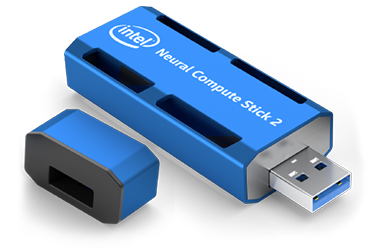
\includegraphics[width=0.3\linewidth]{fig/NCS2-specs}\\
	\footnotesize forrás:software.intel.com/en-us/neural-compute-stick
	\caption{Neural Compute Stick 2 gyorsító} 
	\label{fig:ncs2-specs}
\end{figure}

\subsection{Az NCS2 használata OpenVINO keretrendszerben}
%Az alábbiak alapját az Intel OpenVINO eszközkészletének dokumentációja adja.\cite{web:OpenVINO} A dokumentációban a felépített neurális hálózatokra  modell néven hivatkoznak, amit most én is átveszek.
Az OpenVINO eszközkészletéről részletes és nyílt hozzáférésű dokumentációt ad az Intel. \cite{web:OpenVINO} A felépített neurális hálózatokra a modell szó használata általános, így a dokumentáció is így nevezi azokat.

Az OpenVINO eszközkészlet alkalmas arra, hogy gyorsan készítsünk olyan alkalmazásokat, melyek %valamilyen módon emulálják az emberi látást
kamera szenzor adatainak valós idejű feldolgozását végzik. Képesek vagyunk segítségével az NCS2-n kívül más Intel gyártmányú hardverrel dolgozni, például Intel CPU-n és integrált GPU-n. Továbbá népszerű keretrendszereket támogat, mint a TensorFlow, Caffe, MXNet vagy az ONNX. Az eszközkészlet komponensekei közül az alábbiakat emelném ki:
\begin{description}[noitemsep]
	\item[Inference Engine] C++ és Python API, aminek segítségével különböző gyorsítókártyák megszólíthatók egységes módon.
	\item[Model Optimizer] parancssoros alkalmazás modelleket definiáló állományok átkonvertálására. Ahhoz, hogy a különböző keretrendszerekben megalkotott modelleket egységesen tudja kezelni az Inference Engine, szükség van azok átkonvertálására egy platformfüggetlen struktúrába.
	\item[OpenCV] az OpenCV közösségi fejlesztésű verziójának Intel hardverekre fordított változata.
\end{description}

Az OpenVINO-val való munka folyamatának három fő lépése van:
\begin{enumerate*}[label={}, font=\bfseries]
	\item Betanított Neurális hálózat beszerzése vagy implementálása;
	\item a hálózat átkonvertálása a Model Optimizer-rel;
	\item Inference Engine-re épülő program implementálása, mely beolvassa az átkonvertált állományokat és átadja a neurális hálózat modelljét a célhardvernek;
\end{enumerate*}

\subsubsection{Modell átkonvertálása}
Mint már korábban említettem a platform különböző neurális hálózatok implementálására kifejlesztett keretrendszereket támogat. Ezek a keretrendszerek képesek a definiált és betanított hálózatokat valamilyen állomány formátumban elmenteni. Hogy ezeket az állományokat minden gyorsító eszközön egységesen legyen képes kezelni az \emph{Inference Engine} szükséges az állományokat átkonvertálni a \emph{Model Optimizer} segítségével. Ez egy Python-ban írt kereszt-platformos parancssoros alkalmazás, mely a beolvasott modell állományokban tárolt hálózatot elmenteni egy \emph{közbenső reprezentációvá}\footnote{Intermediate Representation (IR)}, melyre a továbbiakban \emph{IR-ként} fogok hivatkozni. Az átkonvertálás során a Model Optimizer analizálja a modellt\footnote{betanított, kvázi használatra kész neurális hálózat} és olyan korrekciókat hajt végre rajta, hogy optimális módon hajtódjon végre az egyes gyorsítókon. 

Egy TensorFlow-ban implementált neurális hálózat átkonvertáláshoz az alábbi lépéseket kell végrehajtani:
\paragraph*{Model Optimizer konfigurációja}
	Az alkalmazás előre elkészített szkriptekkel települ a különböző keretrendszerekhez történő konfigurációhoz. A szkriptek a \url{<main directory>/deployment_tools/model_optimizer/install_prerequisites} könyvtárban találhatóak. TensorFlow-val való munkához az \verb|install_prerequisites_tf.sh| -- Windows operációs rendszeren ugyanezen fájlnéven \verb|.bat| kiterjesztéssel -- konfigurációs szkriptet kell lefuttatni.

\paragraph*{TensorFlow modell befagyasztása}
	Ez egy keretrendszer specifikus lépés. Amikor Python-ban definiáljuk a hálózatot, rendszerint elmentjük azt egy \emph{inference graph} fájlban. Ez általában olyan módon történik, hogy a hálózat tanítható marad, tehát annak paraméterei, mint változók tárolva vannak az állományban. A Model Optimizer csak úgy tud dolgozni ezen az állományon, ha az úgymond be van \emph{fagyasztva}. A keretrendszerben befagyasztott modell kimentésének műveletét a következő kódrészlet mutatja:
	\begin{lstlisting}[language=Python]
	import tensorflow as tf
	from tensorflow.python.framework import graph_io
	
	frozen = tf.graph_util.convert_variables_to_constants(sess, sess.graph_def, ["output_node"])
	graph_io.write_graph(frozen, './', 'model.pb', as_text=False)
	\end{lstlisting}
	ahol:
	\begin{description}
		\item[\PVerb{sess}] egy TensorFlow \verb|Session| példánynak a referenciaváltozója
		\item[\PVerb{["output\_node"]}] a kimeneti csomópontok nevének listája. Egy befagyasztott hálózat csak azokat a csomópontokat fogja tartalmazni a az eredeti \verb|sess.graph_def|;
		\item[\PVerb{'model.pb'}] a létrehozandó modell fájl neve;
		\item[\PVerb{as\_text}] boolean típusú változóval megadható, hogy a \verb|write_graph| metódus a bináris vagy karakteres formátumban írja ki a gráfot.
	\end{description}

\paragraph*{Modell átkonvertálása}
	Ennél a pontnál használjuk a Model Optimizer-t, azaz ekkor történik meg a konverzió. Az alkalmazás a \url{<főkönyvtár>/deployment_tools/model_optimizer} könyvtárba települ. Hogy a \verb|model.pb| állományunkat átkonvertáljuk a következő parancsot kell kiadni:
	\begin{verbatim}
		python3 mo_tf.py --input_model model.pb
	\end{verbatim}
	A kimenet maga az IR, két állomány: egy xml kiterjesztésű fájl, amiben a hálózat topológiája van definiálva és egy bináris fájl, ami a hálózat paramétereit -- súlyait és küszöbértékeit -- tartalmazza. 
	A program további argumentumaival specializálhatjuk a konvertálás folyamatát.

\subsubsection{Inference Engine}
Az OpenVINO eszközkészlet tartalmaz egy futtatókörnyezetet az \emph{Inference Engine-t}, egy programkönyvtár csomagot melynek központi része a \verb|libinference_engine.so|\footnote{Windows operációs rendszeren természetesen .dll kiterjesztésű és a fájlnév nem tartalmazza a "lib" karaktersort és ez igaz a többi programkönyvtár elnevezésére is} könyvtár. A könyvtárcsomag C++ nyelven íródott, melyhez létezik C++ és python alapú API. Az utóbbihoz készült API szerényebb funkcionalitással bír. Feladati az IR-ben tárolt modell beolvasása, az következtetés (inference) optimalizálása a célhardveren történő végrehajtáshoz  és annak futtatása. A hardvercsoportokkal történő kommunikációs eljárások külön programkönyvtárakba -- ahogy a dokumentáció hivatkozik rájuk \emph{pluginokba} -- lettek szervezve.
\begin{table}[h]
	\centering
	\begin{tabular}{ p{0.3\textwidth} | p{0.63\textwidth} }
		GPU plugin\\(libclDNNPlugin.so) & Intel HD Graphics és Intel Iris Graphics  \\ \hline
		CPU plugin\\(libMKLDNNPlugin.so) & Intel Xeon AVX2 és AVX512 utasításkészlettel, Intel Core AVX2 utasításkészlettel, Intel Atom SSE utasítással \\ \hline
		FPGA plugin\\(libdliaPlugin.so) & Intel Vision Accelerator %Design?
		eszköz Intel Arria 10 FPGA-val (Speed Grade 1 és 2), Intel Programmable Acceleration kártya Intel Arria 10 GX FPGA-val \\ \hline
		VPU plugin\\(libmyriadPlugin.so) & NCS és NCS2, Intel Vision Accelerator %Design?
		eszközök Myraid processzorral\\ \hline
		GNA plugin\\(libGNAPlugin.so) & Intel Speech Enabling Developer Kit, Amazon Alexa Premium Far-Field Developer Kit, Intel Pentium Silver J5005, Intel Celeron J4005, Intel Core i3-8121U \\ \hline
		Multi-Device plugin\\(libMultiDevicePlugin.so) & egy modell több eszközön történő parallel inferenciájára\\ \hline
		Heterogenous plugin\\(libHeteroPlugin.so) & modell automatikus szétosztása több eszközre (akkor szükséges, ha néhány hálózati réteg típust nem minden eszköz támogat)
	\end{tabular}
	\caption{Plugin típusok és támogatott hardverek}
	\label{table:IEplugins}
\end{table}

%Az Inference Engine használatával Python nyelven ismerkedtem meg, így alább ezen nyelvi API használatát mutatom be.
A fejlesztés során is használt python API-n keresztül mutatom be az Inference Engine-t. Az interfészt a következő osztályok szolgálatatják:
\begin{description}[noitemsep]
	\item[\PVerb{ExecutableNetwork}] osztály reprezentál egy modell példányt, amit betöltöttük a pluginba és készen áll az inferenciára;
	\item[\PVerb{IECore}] egy Inference Engine objektum. Segítségével egy egységes interfészen keresztül kezelhetjük a pluginokat;
	\item[\PVerb{IENetLayer}] tartalmazza a főbb információkat a modell rétegeiről, továbbá eszköz a rétegek néhány paraméterének módosításához;
	\item[\PVerb{IENetwork}] minden információt tartalmaz az IR fájlokból beolvasott modellről, és annak paramétereinek módosítását teszi lehetővé;
	\item[\PVerb{IEPlugin}] a plugin-ok fő interfésze. Célja, hogy inicializálja és bekonfigurálja a plugin-t;
	\item[\PVerb{InferRequest}] egy interfészt kínál a következtetés kérésére az  \verb|ExecutableNetwork| osztályon keresztül, továbbá kezeli a predikció végrehajtását és a kapott adatokat;
	\item[\PVerb{InputInfo}] a modell bemeneti rétegének tulajdonságait tartalmazza: \verb|layout| karaktersorozat, a (bemeneti) tenzor elrendezése\footnotemark, \verb|shape| szám n-es a tenzor alakja, \verb|precision| az adatok számábrázolás szerinti típusa;
	\footnotetext{Elrendezés: a tenzorként reprezentált minták tömbjében az adatok milyen elrendezésben szerepelnek. Például egy képfeldolgozáshoz használt hálózat bemeneti rétege esetén az 'NHWC' elrendezés azt jelenti, hogy a beolvasott tömb 1. tengelye mentén a mintákon(sample Number) való bejárást, 2. és 3. tengelye mentén a magassági(Height) és szélességi(Width), negyedik tengelye mentén a színcsatornák(Channel) szerinti bejárást végezhetünk}%\enlargethispage{-\baselineskip}
	\item[\PVerb{LayersStatsMap}] a Python \verb|dict| osztályának leszármaztatása, mely újraimplementálja a \verb|update()| metódust, hogy módosítható legyen a rétegek finomhangolásának statisztikái;
	\item[\PVerb{LayerStats}] a rétegek finomhangolási statisztikáinak konténere;
	\item[\PVerb{OutputInfo}] a modell bemeneti rétegének tulajdonságait tartalmazza hsonlóan az \verb|InputInfo| osztályhoz;
\end{description}

Egy elemi alkalmazás implementációjához, mely inferenciát végez az NCS2 eszközön szükség van az \verb|IENetwork| és \verb|IECore| vagy \verb|IEPlugin| osztályokra továbbá létrejön egy \verb|ExecutableNetwork| egyed, amivel az hálózatot futtatjuk. %A modell feltöltése az eszközre, majd a hálózat futtatása a \ref{lst:IEPython}~kód szerint tehető meg.
A modell feltöltése az eszközre, annak alkalmazásban történő futtatását az eszközön a \ref{lst:IEPython}~kód szemlélteti.
\begin{minipage}{\textwidth}
	\begin{lstlisting}[language=Python,caption=Inference Engine használata PYthon-ból ]
from openvino.inference_engine import IENetwork, IEPlugin
net = IENetwork(model= '<dir>/model.xml', weights= '<dir>/model.bin')
plugin = IEPlugin(device= 'MYRIAD')
exec_net = plugin.load(network= net)
i_layer_key = list(net.inputs.keys())[0]

if net.inputs[i_layer_key].shape == list(samples.shape) :
	res = exec.net.infer(inputs={i_layer_key : samples})
	\end{lstlisting}\label{lst:IEPython}
\end{minipage}
%A model.xml fájl több input réteget is tartalmazhat (type="Input"), ezért az IENetwork inputs mezeje egy olyan dict, aminek kulcsa az input rétegek "name" mezejével, azaz a nevével egyezik, az érték pedig egy InputInfo objektum
Az \verb|IEPlugin| rendelkezik egy \verb|load()| metódussal, mely egy \verb|IENetwork| objektumtól megkapja a hálózat adatait és példányosít egy \verb|ExecutableNetwork| egyedet. Ezen objektum \verb|infer()| metódusával végeztethetjük az inferenciát szinkron módon. Lehetőség van aszinkron üzemmódra az \verb|async_infer()| metódussal. Mindkét metódus használata esetén át kell adni egy táblázat típusú paramétert (Python \verb|dict| osztály) melynek kulcsértékei a bemeneti rétegek nevei (ez egyezik az IENetwork inputs attribútumának kulcsával), a kulcsokhoz rendelt értékek pedig a minták megfelelő alakú, \verb|numpy.ndarray| típusú tenzora. A \verb|res| változó szintén egy táblázat lesz, amiben a kimeneti rétegek neveihez, mint kulcsokhoz van rendelve a következtetés eredménye. 


\section{Google Edge TPU}
Az Intelhez hasonlóan a Google is tervezett célprocesszort és hozzá fejlesztő panelt, mély tanulást alkalmazó projektekhez. A Google Edge TPU-ról és a Coral USB Accelerator-ról a Heartbeat internetes magazinban megjelent cikkben értesültem.\cite{web:GoogleEdge} A Google TPU-ról szerzett ismereteim a wikipédia ,,Tensor Processing unit'' cikkéből szereztem.\cite{wiki:TPU}

\begin{figure*}[h]
	\centering
	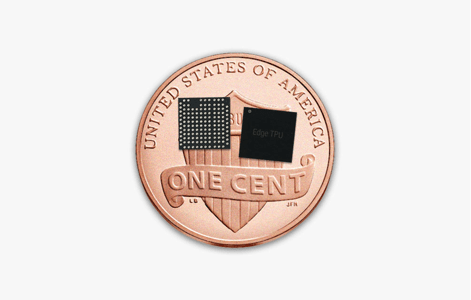
\includegraphics[width=0.4\textwidth]{fig/penny-edge-tpu}\\
	\footnotesize forrás:cloud.google.com/edge-tpu/
	\caption{Edge TPU}
	\label{fig:EdgeTPU}
\end{figure*}
\begin{figure*}[h]
	\centering
	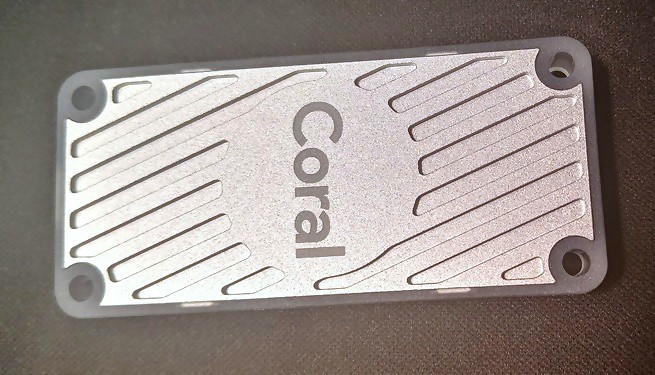
\includegraphics[width=0.4\textwidth]{fig/Coral_USBAccelerator}\quad
	\caption[Coral USB Accelerator]{Az Edge TPU-t építették az USB interfésszel ellátott Coral USB Accerleratorba. \footnotesize forrás:\cite{web:GoogleEdge}}
	\label{fig:coralusbaccelerator}
\end{figure*}

A Google a \emph{Tensor Processing Unitot}, egy saját fejlesztésű alkalmazásspecifikus integrált áramkört használ a neurális hálózatokkal kapcsolatos számítások optimalizálására. Ezek lényegében mátrix műveletekre számítására fejlesztett processzorok CISC utasításkészlettel. Három generációt ért meg, az első még csak 8-bites egészeken tudott műveleteket végezni, azonban már a második generáció képes volt lebegőpontos számításokra is. A Tensor processing unit-okkal felszerelt gyorsítókártyákat a Google saját adatközpontjaiban használja főként és elérhetővé teszi őket a \emph{Google Cloud Platform} nevű szolgáltatásán keresztül. Nevéből adódóan a kártya architektúrája lehetővé teszi, hogy  tenzorműveletek tudjanak hatékonyan végrehajtani, utasításkészletük kifejezetten támogatja a neurális hálózatokat. Ilyen művelet a konvolúció és az \ref{sect:neuralNetworkTheory} alfejezetben tárgyalt aktváló függvények alkalmazása a mátrix szorzáson túl.

Az Edge TPU a cég szerverei által használt TPU-hoz viszonyítva kisebb méretben és energiafogyasztásban. Ugyan azt az igényt igyekszik kielégíteni, mint a korábban bemutatott Myriad X processzor. Azzal összehasonlítva viszont képes neurális hálózatok tanítására is korlátozott mértékben. Az Edge TPU részét képezi a Google Coral eszközkészletének, mellyel alternatívát nyújtanak a felhőalapú Cloud AI szolgáltatással szemben. A Coral különböző fajtájú hardvert nyújt a felhasználóknak, mindegyik központi eleme az Edge TPU. Az eszköz programozásához használható API-t az Edge TPU Python könyvtár (\verb|edgetpu| Python modul) valósítja meg, amely képes TensorFlow Lite-ban alkotott betanított neurális hálózatok futtatására. A könyvtár kulcsfontosságú interfészeit a következő osztályok képezik.Képosztályozási feladatokhoz a \verb|ClassificationEngine| használatos, vizuális objektumazonosításra a \verb|DetectionEngine|. Az \verb|ImprintingEngine| és \verb|SoftmaxRegression| az ún. \emph{transzfer tanuláshoz} alkalmazható, vagyis előre betanított hálózatok a feladatnak megfelelő újratanítását végezhetjük el vele.


\section{Új gyorsítók: Intel Nervana Neural Network Processor}

Az Intel idén augusztusban mutatta be a Hot Chips konferencián kifejezetten mély tanulásra Spring Crest és Spring Hill kódnevek alatt fejlesztett  rendszerchipeket, a Neural Network Processor for Training-et (NNP-T) és a Neural Network Processor for Inference-et (NNP-I)\cite{web:IntelNews2019}. Mint nevük is mutatja ezek kifejezetten mély tanulás gyorsításra lettek fejlesztve és úgy tervezték őket, hogy jól skálázható rendszert alkossanak. Ezeket a hardvereket a konferencián elmondottak alapján mutatnám be.\cite{yt:nnpt}\cite{yt:nnpi} Ebben az alfejezetben szereplő ábrák a konferencián levetített fóliákból származnak.\cite{yang-nnpt}\cite{Wechsler-nnpi}

\subsection[NNP-T]{Neural Network Processor for Training}
Az NNP-T egy egylapkás rendszer vagy rendszerchip, melynek fejlesztésénél fontos szempont volt az egyensúly a számítási teljesítmény, a perifériák közötti kommunikáció  sebessége és memória használat között. Ezt támogatja 
a lapka memóriájába már betöltött adatok minél hatékonyabb újrafelhasználásának elősegítése, továbbá a kötegelt adatfeldolgozás optimalizálása. Könnyen skálázható rendszert lehet építeni belőle, ugyanis ezt beépített megoldások segítik. A jövőbeli munkafolyamatokat is támogatására a számítási egységek utasításkészlete programozható.

\subsubsection{Hardver tulajdonságai}
\paragraph[Soc]{Rendszerchip}
A chip 4. generációs 16 sávos PCIe végponttal rendelkezik. A nagy memóriakapacitás lehetőségét lapkán 4 darab HBM2\footnote{High Bandwidth Memory: DRAM modulok térben egymásra pakolását alkalmazó RAM interfész típus. HBM2 esetén a legnagyobb kapacitás 8GB lehet egy tokban. Leginkább videó kártyákban használatos } memória foglalattal oldották meg. A lapkák közötti kommunikációra SerDes interfész 64~sávval is implementálva lett.
A számításokat 24~darab tenzor processzormag végzi(TPC), és a vállalat szerint számítási kapacitásuk összesen 119~TOP/s (billió utasítás másodpercenként).A lapkán elhelyeztek 60~MB osztott memóriát is.
\begin{figure}[H]
	\centering
	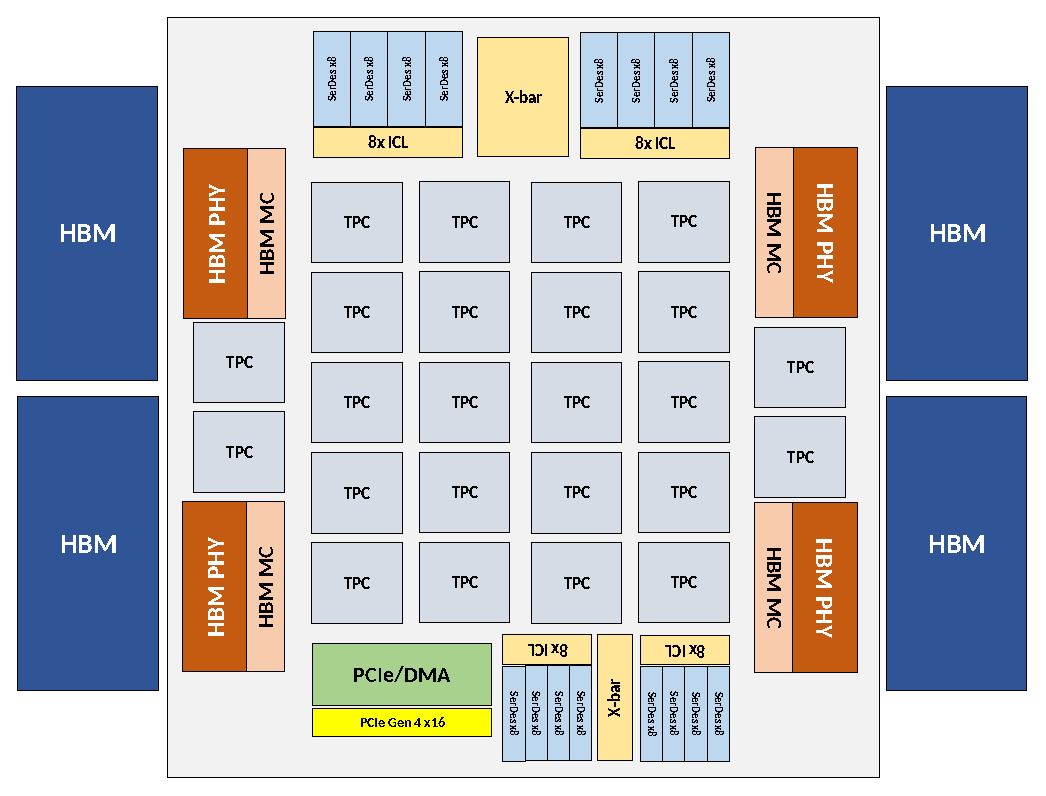
\includegraphics[width=0.7\linewidth]{NNP-T_soc}
	\caption[SoC]{Az NNP-T egylapkás rendszer (SoC) felépítése}
	\label{fig:nnp-tsoc}
\end{figure}

\paragraph{Tenzor processzor (TPC)}
Egy TPC magon belül két darab mátrixszorzó tömb van, melyek egyenként 32$\times$32-es méretű mátrixok tud szorzást végezni, a konvolúció műveletet pedig külön egység végzi. Minden mag továbbá rendelkezik 2,5~MB Cache memóriával, melyek sávszélessége 1,4~TB/s. A \ref{fig:TPC} ábrán látható zöld színnel jelzett útválasztó a magok közötti kommunikációért felelős. 
\begin{figure}[H]
	\centering
	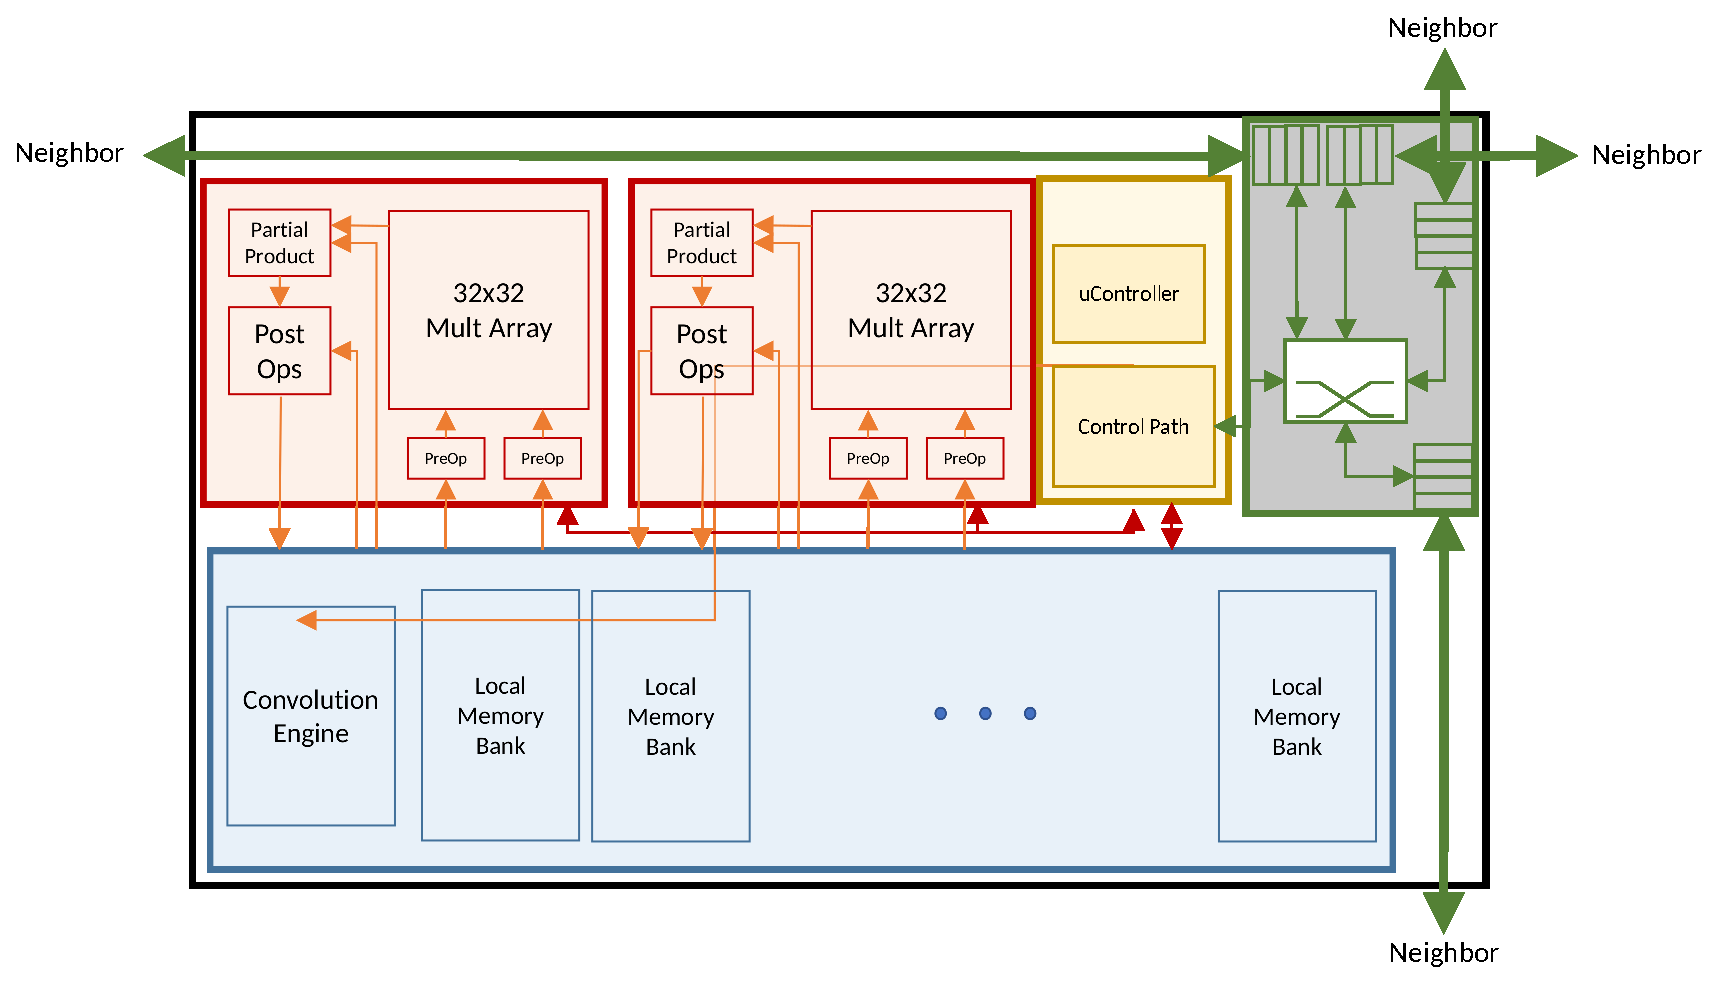
\includegraphics[width=0.7\linewidth]{tensor-processing-cluster_TPC}
	\caption[TPC]{Egy TPC felépítése}
	\label{fig:TPC}
\end{figure}

\paragraph{hardverkártya tulajdonságai}
%TSMC CLN16FF+
%680mm 2 , 1200mm 2 interposer
%27 Billion Transistors
Az Intel az NNP-T rendszerchipet egyedi PCIe és OAM alaktényezőjű kártyán fogja forgalmazni, melyre egy rendszerchipet szerelnek összesen 32~GB HBM2-2400 típusú memóriával -- melynek elméleti sávszélessége 1,22~TB/s -- BGA tokozásban.
A rendszerchip órajele az 1,1GHz-et is elérheti. A kártya 4. generációs PCI Express x16, valamint SPI, I2C csatolófelülettel és általános célú I/O kivezetéssel rendelkezik. A központi egység léghűtésű átlagos használat esetén 150 és 250~W közötti fogyasztással. A kártyán kivezetésre került 64~SerDes sáv, melynek aggregált sávszélessége 3,58~Tb/s. Ezen interfész segít megvalósítani több lapka összehangolt működését, mellyel maximum 1024 csomópontot lehet összekötni úgy, hogy azok összes TPC magja egy nagy hálózatként kezelhető, ezzel elérve a masszív párhuzamosítást. 

\subsubsection{Az NNP-T programozásához használatos szoftver együttes}
Az alkalmazásfejlesztés az ilyen rendszerchipekkel szerelt kártyákra egyedi eszközkészlettel lehetséges. A vállalat ajánl egy teljes fejlesztői szoftverkészletet nyílt forrású komponensekkel. A \ref{fig:nnp-tSwStack}~ábra az egyes komponenseket hardver és felhasználó közötti viszonya szerint rétegezve mutatja be. Ezek közül az nGraph-ot és a magas szintű keretrendszerek közül a TensorFlow-t, már bemutattam korábban, illetve pár szóban összefoglalom az Argon programkönyvtárat.
%nGraph: Hardware agnostic deep learning library and compiler for DL platform developers. -> Provides common set of optimizations for NNP-T across DL frameworks
%Argon: NNP-T DNN compute and communication kernel library
%Low-level programmability: NNP-T kernel development toolchain w/tensor compiler
\begin{figure}[H]
	\centering
	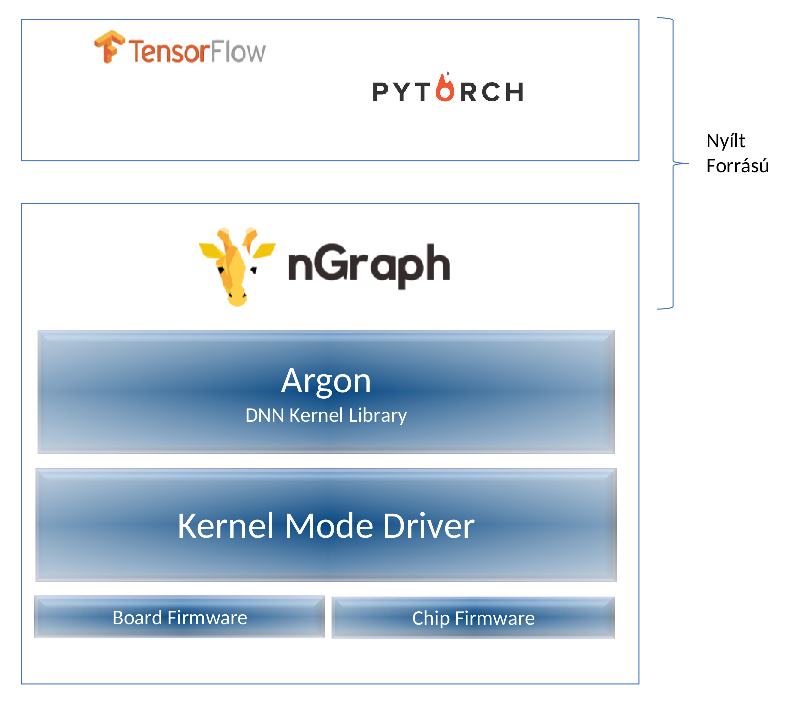
\includegraphics[width=0.5\linewidth]{nnp-t_softwares}
	\caption[Szoftverek]{Fejlesztéshez használható szoftveregyüttes}
	\label{fig:nnp-tSwStack}
\end{figure}

\subsubsection{NNP-T Programozási modell}
Az Utasításkészlet szintjén is neurális hálózatokra lett optimalizálva a rendszerchip azzal, hogy a hálózat tanításakor alkalmazandó tenzor műveletekhez natív utasítások tartoznak, úgy mint transzponálás, tenzor darabolása, stb. Az utasításkészlet is ezen utasításokra van korlátozva, azonban ez bővíthető egyedi mikrokontroller kutasításokkal. A bővíthetőség azt a célt szolgálja, hogy a jövőbeli mély tanulásra épülő munkafolyamatok támogatottsága is megoldható legyen utasítás szinten. 
Az Intel hierarchikus elosztott programozási modellt használ, ami jól skálázható, így alkalmazható egy rendszerchip TPC magjaira, vagy akár több lapka együttes programozáskor. Ezt segíti, hogy a magok közti kommunikáció és szinkronizáció elemi utasításai konzisztensek lapkán belül és több lapka között.
Azon túl, hogy a hardver az adatokat tenzoronként kezeli, a tenzorokon belüli elemi változókat Bfloat16\footnote{Az IEEE 754 félszeres, azaz 16~bites pontosságú lebegőpontos típustól annyiban tér el, hogy az exponens 5 helyett 8~bites. Ez az Intel állítása szerint azon túl, hogy memória hely takarékos, tanításkor jól konvergáló változókat biztosít} és 32~bites lebegőpontos típusként tudja értelmezni

\subsection[NNP-I]{Neural Network Processor for Inference}
Betanított neurális hálózatok futtatására alkalmazható rendszerchip, melyet az NNP-T-vel együtt kezdett el fejleszteni a vállalat. Ennél a lapkánál a cél a kis fogyasztás volt. A gyártó szerint Wattonkénti 4,8~billió számítást képes végezni másodpercenként. A számítási teljesítmény a fogyasztás hangolásával természetesen változó. (Jelenleg M.2 és PCIe alaktényezőjű kártyákon forgalmazzák. Előbbi 12~wattos teljesítményű, míg az utóbbi teljesítménye 75~W. Számítási kapacitásuk 50 és 170~TOP/s)

Hasonlóan az NNP-T-hez ez a rendszerchip is egyedi processzormagokat tartalmaz, összesen 12-t. A mag megnevezése \emph{Inference Compute Engine}, röviden ICE. Az lapka (\ref{fig:nnp-isoc}~ábra) kiegészül még 24~MB cache memóriával, melyen az összes mag osztozik.
%Egy ICE elég önálló ahhoz, hogy egy egyszerűbb hálózatot egészben lmodellezzen, de persze az ICE magok képesek összedolgozni
Az ICE magok mellett két Intel IA Core processzormag is részét képezi a rendszerchipnek. Ezek párban az ICE-k munkáját hangolják össze a fordítótól érkező utasítások alapján, -- ide kapcsolódik, hogy \emph{Ahead Of Time} fordítás végezhető az eszközre -- tehát a programozó által közvetlenül ez a két processzormag elérhető. Egy ICE két számítást végző blokkból áll: egy \emph{Deep Learning compute grid}-nek nevezett több számítási egységből álló hálózatból, -- melyek a neurális hálózatok modellezése során igényelt műveletek javát végzik -- illetve egy programozható vektor processzorból AVX és VNNI utasításkészlettel. A vektor processzor jóvoltából tetszőleges utasításokkal bővíthető a mag.

\begin{figure}[H]
	\centering
	\begin{subfigure}{0.4\textwidth}
		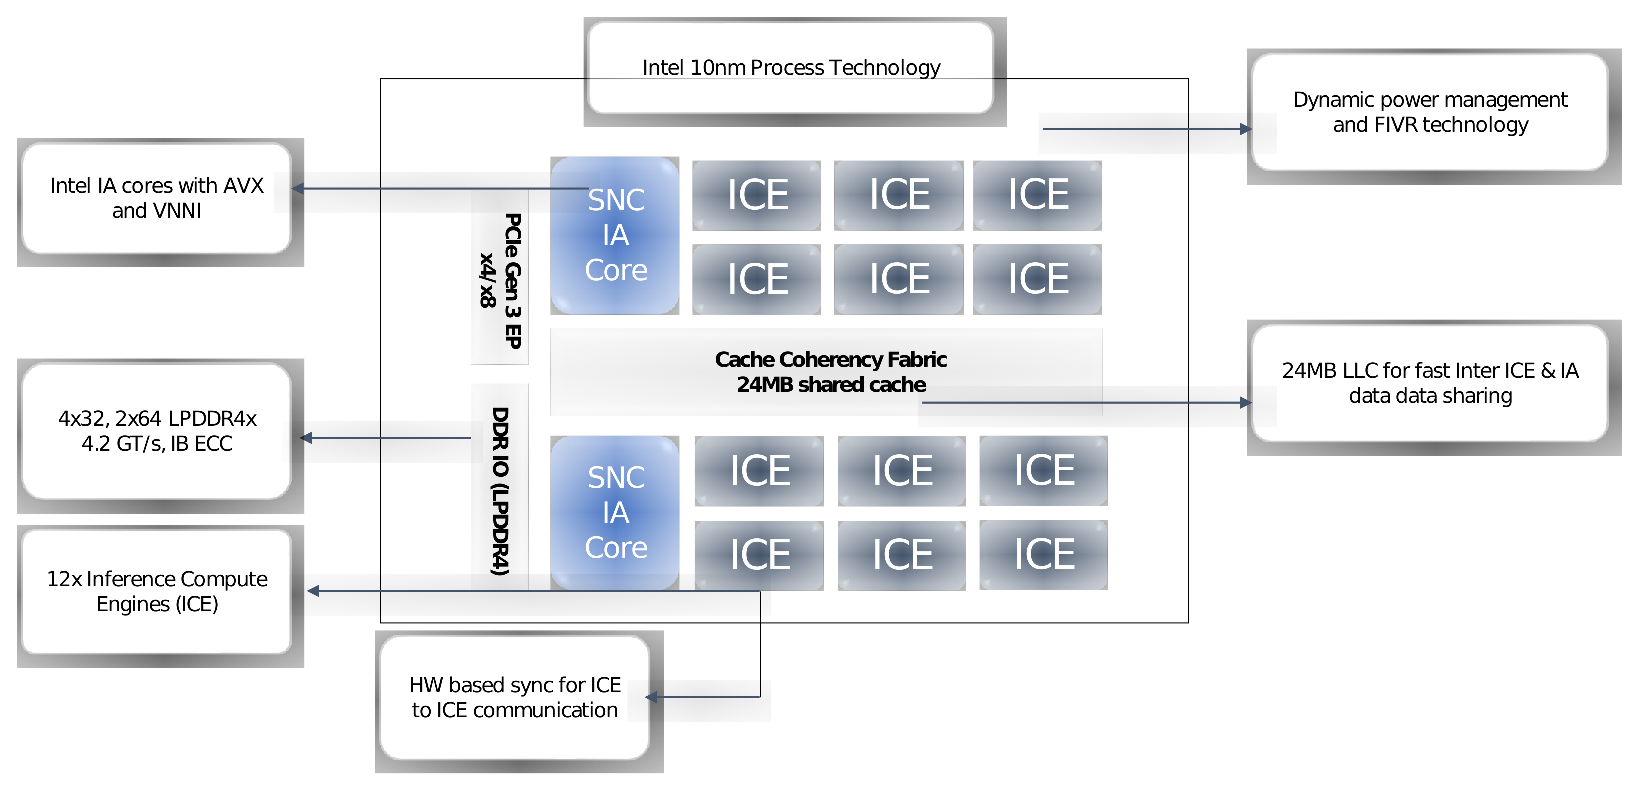
\includegraphics[width=\textwidth]{fig/NNP-I_soc}
		\caption{Az SoC logikai felépítése}
		\label{fig:nnp-isoc}
	\end{subfigure}
	\quad
	\begin{subfigure}{0.4\textwidth}
		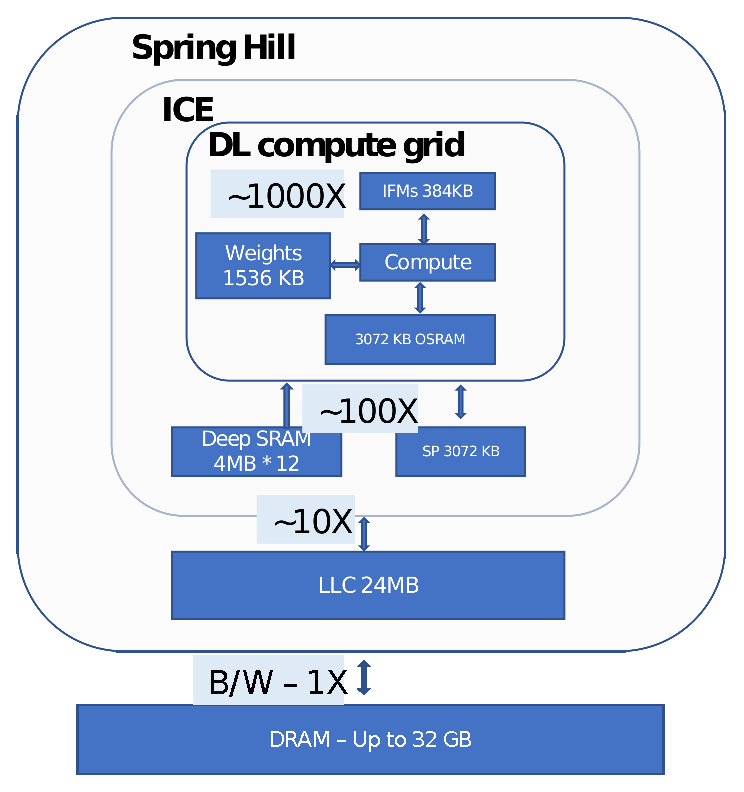
\includegraphics[width=\textwidth]{fig/NNP-I_memManagement}
		\caption{Memória menedzsment}
		\label{fig:nnp-imem}
	\end{subfigure}
	\caption{}
	\label{fig:nnp-i}
\end{figure}

Egy ICE 4~MB lokális SRAM memóriát kapott. Ezen ICE magok képesek 16 bites lebegőpontos valamint 8, 4, 2 és 1~bites egész változókat kezelni. Az NNP-I lapka 3. generációs PCIe (x4 vagy x8) végponttal kapcsolódik a befogadó kártyához, továbbá egy LP-DDR4 memória ültethető a hordozó lapkára az S . Azért, hogy az adatmozgatást minimalizálják a memória allokáció 4 szinten van rendezve hierarchikusan, ahogy az \ref{fig:nnp-imem}~ábrán látható. Ezt a rendszerchipet ugyanazzal a szoftver együttessel tudjuk programozni, mint az NNP-T SoC-t.